\documentclass{file/TA-ITS}
%Ridho Nur Rohman Wijaya

\makeatletter
\def\cleardoublepage{\clearpage%
	\if@twoside
	\ifodd\c@page\else
	\vspace*{\fill}
	\hfill
	\begin{center}
		\emph{ }
	\end{center}
	\vspace{\fill}
	\thispagestyle{empty}
	\newpage
	\if@twocolumn\hbox{}\newpage\fi
	\fi
	\fi
}
\makeatother
\newtheorem{definisi}{Definisi}[section]
\newtheorem{teorema}[definisi]{Teorema}
\newtheorem{thm}{Teorema}[section]
\newtheorem{lemma}[definisi]{Lemma}
\newtheorem{lemmas}[thm]{Lemma}
\newtheorem{cor}[definisi]{Akibat}
\theoremstyle{definition}
\newtheorem{con}[definisi]{Contoh}
\theoremstyle{definition}
\theoremstyle{plain}
\newtheorem{prop}[definisi]{Proposisi}
\renewcommand{\proofname}{Bukti}
\renewcommand{\thethm}{\arabic{chapter}.\arabic{thm}}

\newcommand{\norm}[1]{\left\|#1\right\|} % Fungsi norm (||x||)

\newcommand\firstPar{0.75cm} % Indentasi 0.75cm pada tiap paragraf (manual untuk hspace)
\setlength{\parindent}{0.75cm} % Indentasi 0.75cm pada tiap paragraf

\usepackage{fancyhdr}
\pagestyle{fancy}
\renewcommand{\headrulewidth}{0pt}
\fancyhf{}
\usepackage{ifthen}
\fancyfoot[R]{\thepage}

\usepackage[labelsep=quad]{caption}
\captionsetup[table]{skip=5pt}

\usepackage{multirow}
\usepackage{longtable}

%%% Pewarnaan code
\usepackage{color}
\usepackage{listings}

\definecolor{codegreen}{rgb}{0,0.6,0}
\definecolor{codeblack}{rgb}{0,0,0}
\definecolor{codepurple}{rgb}{0.58,0,0.82}
\definecolor{backcolour}{rgb}{0.95,0.95,0.92}

\lstdefinestyle{mystyle}{
    commentstyle=\color{codegreen},
    keywordstyle=\color{magenta},
    numberstyle=\tiny\color{codeblack},
    stringstyle=\color{codepurple},
    basicstyle=\ttfamily\footnotesize,
    breakatwhitespace=false,         
    breaklines=true,                 
    captionpos=b,                    
    keepspaces=true,                 
    numbers=left,                    
    numbersep=5pt,                  
    showspaces=false,                
    showstringspaces=false,
    showtabs=false,                  
    tabsize=2
}
%%% Pewarnaan code

\hypersetup{ % Merubah warna link
    colorlinks,
    linkcolor={black},
    citecolor={black},
    urlcolor={black}
}

% \tolerance=1
% \emergencystretch = \maxdimen
% \hyphenpenalty=10000
% \hbadness=1000

\newcommand{\Real}{\mathbb{R}}
\newcommand{\N}{\mathbb{N}}
\newcommand{\Z}{\mathbb{Z}}
\newcommand{\Q}{\mathbb{Q}}
\newcommand{\defeq}{\overset{\mathrm{def}}{=}}

\begin{document}

% input data
\Judul{Optimisasi Jadwal Jaringan Bus di Terminal Purabaya Menggunakan Aljabar Max-Plus}

\JudulEng{Optimization of Bus Network Scheduling at Purabaya Terminal Using Max-Plus Algebra}

\Nama{Teosofi Hidayah Agung}

\NamaKecil{Teosofi Hidayah Agung}

\NRP{5002221132}

\Departemen{Matematika}

\Department{Mathematics}

\BidangStudi{Aljabar dan Analisis}

\Bulan{November} % Masuk lembar pengesahan

\Tahun{2024}

\TanggalDisetujui{22 November 2024} % Masuk lembar orisinilitas

\Fakultas{Sains dan Analitika Data}

\SingkatanFakultas{FSAD}

\Faculty{Scientics}

\SingkatanFakultasEng{SCIENTICS}

\Pembimbing{Pembimbing 1}
          {} % Isi {} untuk pembimbing 2
		   

\NIPPembimbing{NIP}
{} % Isi {} untuk pembimbing 2
              
              
\Penguji{Penguji 1}
        {Penguji 2}
        {Penguji 3}

\NIPPenguji{NIP Penguji 1}
           {NIP Penguji 2}
           {NIP Penguji 3}
\Kadep{Nama Kadept}

\NIPKadep{NIP Pak Kadept}
\BagianAwal
\LembarJudul
\LembarPengesahan
%%%%%%%%%%%%%%%%%%%%%%%%  Abstrak  %%%%%%%%%%%%%%%5%%%%%%%%%%

\begin{Abstrak}
Transportasi publik merupakan salah satu komponen penting dalam mendukung mobilitas masyarakat perkotaan. Terminal Purabaya memiliki peran strategis dalam sistem transportasi di Surabaya, namun pengelolaan jadwal bus yang kurang optimal dapat menyebabkan ketidakefisienan waktu tunggu penumpang dan pengoperasian bus. Penelitian ini bertujuan mengoptimalkan jadwal jaringan bus di Terminal Purabaya menggunakan pendekatan aljabar max-plus. Pendekatan ini memodelkan jadwal sebagai sistem linier max-plus yang mempertimbangkan waktu siklus (\textit{cyclicity}) dan waktu transient untuk memastikan efisiensi. Hasil simulasi diharapkan dapat meningkatkan akurasi dan efisiensi operasional bus.

\katakunci{Optimasi jadwal, aljabar max-plus, jaringan bus, efisiensi transportasi.}
\end{Abstrak}

\begin{Abstract}
Public transportation is a critical component supporting urban mobility. Purabaya Terminal plays a strategic role in Surabaya's transport system; however, suboptimal bus schedule management leads to inefficiencies in passenger waiting times and bus operations. This study aims to optimize the bus network schedule at Purabaya Terminal using the max-plus algebra approach. This approach models the schedule as a max-plus linear system, considering cyclicity and transient times to ensure efficiency. The simulation results are expected to enhance the accuracy and operational efficiency of bus services.

\keywords{Schedule optimization, max-plus algebra, bus network, transport efficiency.}
\end{Abstract}

%%%%%%%%%%%%%%%%%%%%%%%%  Abstrak  %%%%%%%%%%%%%%%5%%%%%%%%%%

%%%%%%%%%%%%%%%%%%%%%%%%  Daftar  %%%%%%%%%%%%%%%5%%%%%%%%%%

\DaftarIsi\raggedbottom

\DaftarGambar

\DaftarTabel

\DaftarSimbol
\begin{flushleft}
\begin{tabular}{lrl}

$\oplus$ &:& Operasi \textit{max} dalam aljabar max-plus \\

$\otimes$ &:& Operasi \textit{plus} dalam aljabar max-plus \\

$\varepsilon$ &:& Elemen netral untuk operasi $\oplus$, yaitu $-\infty$ \\

$e$ &:& Elemen netral untuk operasi $\otimes$, yaitu $0$ \\

$\mathbf{A} \otimes \mathbf{x}$ &:& Hasil kali matriks $\mathbf{A}$ dengan vektor $\mathbf{x}$ pada aljabar max-plus \\

$\lambda$ &:& Nilai eigen dalam aljabar max-plus \\

$\mathbb{R}_{\max}$ &:& Himpunan bilangan real diperluas dengan $-\infty$ dalam aljabar max-plus \\

$\mathbb{R}_{\max}^n$ &:& Ruang vektor berdimensi $n$ dalam aljabar max-plus \\

$[\mathbf{A}^k]_{ij}$ &:& Elemen $(i,j)$ dari matriks $\mathbf{A}$ pangkat $k$ \\

\end{tabular}
\end{flushleft}
%%%%%%%%%%%%%%%%%%%%%%%%  Daftar  %%%%%%%%%%%%%%%5%%%%%%%%%%

\BagianInti

%%%%%%%%%%%%%%%%%%%%%%%%  Bab I  %%%%%%%%%%%%%%%5%%%%%%%%%%
\chapter{PENDAHULUAN}
\section{Latar Belakang}
\indent Bus merupakan salah satu transportasi umum yang paling banyak digunakan oleh masyarakat Indonesia, terutama karena keunggulannya dalam menjangkau berbagai wilayah, baik perkotaan maupun pedesaan. Layanan bus tidak hanya melayani kebutuhan transportasi dalam kota, tetapi juga digunakan secara luas untuk perjalanan antar kota dan antar provinsi, terutama bagi mereka yang ingin bepergian ke kota-kota besar untuk bekerja, atau sebaliknya, pulang ke kampung halaman untuk berkumpul bersama keluarga. Popularitas bus sebagai sarana transportasi publik di Indonesia juga didukung oleh biayanya yang relatif terjangkau serta fleksibilitas rutenya yang mencakup area yang tidak selalu terjangkau oleh moda transportasi lain seperti kereta api atau pesawat \cite{Arum2015}.

Terminal Purabaya, yang dikenal sebagai salah satu terminal bus terbesar di Asia Tenggara, memegang peranan penting dalam sistem transportasi publik di Surabaya dan sekitarnya. Terminal ini melayani ribuan penumpang setiap harinya, baik dari dalam kota maupun antarprovinsi. Berdasarkan studi mengenai transportasi publik, pengelolaan terminal bus seperti Purabaya membutuhkan perencanaan yang matang untuk memastikan kelancaran operasi, mengurangi waktu tunggu penumpang, dan meningkatkan efisiensi rute bus. Hal ini sejalan dengan kebutuhan untuk terus mengembangkan sistem transportasi yang lebih terintegrasi dan tepat waktu. Kondisi lalu lintas di sekitar terminal juga menjadi tantangan yang signifikan, karena kemacetan sering terjadi akibat kepadatan kendaraan, terutama di area persimpangan yang dilalui rute bus. Hal ini mempengaruhi jadwal kedatangan dan keberangkatan bus, sehingga penting untuk menerapkan sistem yang dapat meningkatkan efisiensi operasional di terminal \cite{budi2018}.

Sistem transportasi publik, terutama jaringan bus, memainkan peran penting dalam mobilitas masyarakat urban. Efisiensi dalam pengelolaan dan operasi bus sangat bergantung pada kemampuan untuk mengelola antrian penumpang dan waktu kedatangan bus secara efektif. Dalam konteks ini, aljabar max-plus muncul sebagai alat matematis yang menjanjikan untuk memodelkan dan menganalisis antrian dalam sistem transportasi.

Aljabar max-plus, yang telah dikembangkan lebih lanjut dalam beberapa dekade terakhir, merupakan perluasan dari aljabar biasa yang menggantikan operasi penjumlahan dan perkalian dengan operasi maksimum dan penjumlahan. Pendekatan ini sangat berguna dalam memodelkan proses yang melibatkan waktu dan urutan, seperti dalam antrian bus, di mana waktu kedatangan dan waktu tunggu merupakan variabel kunci. Sebagai contoh, penelitian terbaru oleh \citeauthor{butkovic2010maxplus} membahas aplikasi aljabar max-plus dalam sistem penjadwalan dan optimasi waktu, termasuk transportasi publik. Melalui pendekatan ini, kita dapat menganalisis dinamika sistem antrian dan mengoptimalkan pengaturan jadwal bus untuk meminimalkan waktu tunggu penumpang serta meningkatkan kepuasan pelanggan \cite{butkovic2010maxplus}.

Penggunaan aljabar max-plus dalam sistem antrian tidak hanya terbatas pada optimasi jadwal tetapi juga mencakup pengembangan algoritma yang efisien untuk penjadwalan dan pengendalian lalu lintas bus. Penelitian oleh \citeauthor{baccelli} menunjukkan bahwa model max-plus dapat digunakan untuk merepresentasikan interaksi antar kendaraan dalam jaringan transportasi yang kompleks. Dengan memanfaatkan struktur aljabar ini, kita dapat merumuskan solusi yang lebih baik untuk mengatasi masalah antrian, terutama dalam kondisi puncak di mana permintaan penumpang meningkat.

Dengan pertumbuhan populasi dan meningkatnya permintaan akan layanan transportasi publik yang efisien, penelitian lebih lanjut mengenai aplikasi aljabar max-plus dalam antrian bus sangat penting. Penelitian ini tidak hanya bertujuan untuk meningkatkan pemahaman tentang dinamika antrian, tetapi juga untuk memberikan rekomendasi praktis dalam perancangan sistem transportasi yang lebih responsif dan efisien.


\section{Rumusan Masalah}
Berdasarkan latar belakang di atas, penelitian ini mengidentifikasi beberapa masalah yang perlu diselesaikan terkait dengan efisiensi sistem antrian bus di terminal bus, terutama dengan menggunakan pendekatan aljabar max-plus. Rumusan masalah yang akan dibahas dalam penelitian ini adalah sebagai berikut:

\begin{enumerate}
    \item Bagaimana memodelkan sistem antrian bus di terminal menggunakan aljabar max-plus?
    \item Bagaimana mengoptimalkan jadwal kedatangan dan keberangkatan bus untuk meminimalkan waktu tunggu penumpang menggunakan aljabar max-plus?
    \item Bagaimana menerapkan model aljabar max-plus untuk meningkatkan efisiensi operasional dalam kondisi puncak ketika permintaan penumpang meningkat?
\end{enumerate}

Dengan mengatasi rumusan masalah tersebut, penelitian ini bertujuan untuk mengembangkan solusi yang dapat diterapkan pada sistem transportasi publik, khususnya jaringan bus, agar lebih efisien dan tepat waktu.

\section{Batasan Masalah}
Untuk menjaga fokus penelitian dan memperjelas lingkup penelitian ini, terdapat beberapa batasan masalah yang ditetapkan, antara lain:

\begin{enumerate}
    \item Penelitian ini hanya akan memodelkan sistem antrian bus di terminal bus dengan menggunakan pendekatan aljabar max-plus.
    \item Hanya antrian dan jadwal kedatangan/keberangkatan bus yang akan dianalisis, tanpa mempertimbangkan faktor eksternal seperti cuaca, kondisi jalan, atau perubahan kebijakan transportasi.
    \item Studi kasus yang digunakan dalam penelitian ini akan difokuskan pada Terminal Purabaya sebagai salah satu contoh terminal bus besar di Indonesia.
    \item Simulasi yang dilakukan untuk menguji model max-plus akan menggunakan data sekunder yang tersedia dari laporan transportasi publik dan literatur terkait.
\end{enumerate}

\section{Tujuan}
Tujuan dari penelitian ini adalah untuk memberikan solusi yang lebih efisien dalam pengelolaan sistem antrian bus dengan menggunakan metode aljabar max-plus. Secara khusus, penelitian ini bertujuan untuk:

\begin{enumerate}
    \item Mengembangkan model sistem antrian bus yang menggunakan aljabar max-plus untuk merepresentasikan waktu kedatangan dan keberangkatan bus.
    \item Mengoptimalkan jadwal operasional bus di terminal untuk meminimalkan waktu tunggu penumpang.
    \item Menganalisis penerapan model aljabar max-plus dalam meningkatkan efisiensi operasional terminal bus, terutama pada saat jam sibuk dengan permintaan penumpang yang tinggi.
    \item Memberikan rekomendasi praktis untuk pengelolaan sistem transportasi publik yang lebih efisien berdasarkan hasil analisis dan simulasi.
\end{enumerate}

\section{Manfaat}
Penelitian ini diharapkan memberikan beberapa manfaat, baik secara teoritis maupun praktis, di antaranya:

\begin{itemize}
    \item \textbf{Manfaat Teoritis}: Penelitian ini dapat menambah wawasan dan pengetahuan dalam bidang aljabar max-plus, khususnya dalam aplikasinya pada sistem transportasi publik. Model yang dihasilkan juga dapat menjadi dasar bagi penelitian lanjutan dalam bidang optimasi antrian dan penjadwalan.
    \item \textbf{Manfaat Praktis}: Hasil penelitian ini dapat memberikan solusi bagi pengelola terminal bus dalam meningkatkan efisiensi operasional. Dengan penerapan aljabar max-plus, sistem antrian dan jadwal bus dapat dioptimalkan sehingga mengurangi waktu tunggu penumpang dan meningkatkan pengalaman pengguna layanan transportasi publik.
    \item \textbf{Manfaat Kebijakan}: Temuan penelitian ini juga dapat dijadikan sebagai pertimbangan oleh pemerintah atau pihak pengelola transportasi dalam perencanaan dan pengelolaan terminal bus, khususnya untuk meningkatkan efisiensi dan kualitas layanan transportasi publik di Indonesia.
\end{itemize}

\pagebreak
\chapter{TINJAUAN PUSTAKA}

\section{Terminologi Aljabar Max-Plus}
\indent Aljabar max-plus adalah perluasan dari aljabar biasa yang menggantikan operasi penjumlahan dan perkalian dengan operasi maksimum dan penjumlahan, Sebagaimana definisi yang diberikan sebagai berikut:
\begin{definisi}
    Diberikan himpunan $\Real_{\varepsilon} = \Real \cup \{\varepsilon\}$ dengan $\Real$ adalah himpunan bilangan real dan $\varepsilon\defeq-\infty$. Pada $\Real_{\varepsilon}$, didefinisikan dua operasi biner sebagai berikut:
    \begin{flalign}
        a \oplus b &\defeq \max\{a, b\} , \quad \forall a, b \in \Real_{\varepsilon} \label{eq:oplus} \\
        a \otimes b &\defeq a + b , \quad \forall a, b \in \Real_{\varepsilon} \label{eq:otimes}
    \end{flalign}
\end{definisi}
\noindent\cite{baccelli}

Selanjutnya akan ditunjukkan bahwa $\left(\Real_\varepsilon,\oplus,\otimes\right)$ adalah semiring dengan elemen netral $\varepsilon=-\infty$ dan elemen satuan $e=0$. Untuk setiap $a,b,c\in\Real_\varepsilon$, berlaku sifat-sifat berikut:
\begin{enumerate}
    \item \textbf{Komutatif} : $a\oplus b=\max\{a,b\}=\max\{b,a\}=b\oplus a$.
    \item \textbf{Asosiatif} : $(a\oplus b)\oplus c=\max\{\max\{a,b\},c\}=\max\{a,\max\{b,c\}\}=a\oplus\max\{b,c\}=a\oplus(b\oplus c)$.
    \item \textbf{Elemen netral} : $a\oplus\varepsilon=\max\{a,\varepsilon\}=\max\{a,-\infty\}=a$.
    \item \textbf{Elemen satuan} : $a\otimes e=a+0=a$.
    \item \textbf{Distributif} : $a\otimes(b\oplus c)=a\otimes\max\{b,c\}=a+\max\{b,c\}=\max\{a+b,a+c\}=a\oplus b\otimes a\oplus c$.
\end{enumerate}
Notasi $\left(\Real_\varepsilon,\oplus,\otimes\right)$ bisa ditulis sebagai $\Real_{\max}$ \cite{subiono2015minmaxplus}.

\section{Vektor dan Matriks}

\indent Dalam aljabar max-plus, vektor dan matriks didefinisikan dengan menggunakan operasi max-plus, di mana operasi dasar penjumlahan digantikan oleh operasi maksimum (\(\oplus\)) dan perkalian digantikan oleh penjumlahan biasa (\(\otimes\)) \cite{butkovic2010maxplus,heidergott,baccelli}. Definisi untuk vektor dan matriks dalam konteks aljabar max-plus dapat dijelaskan sebagai berikut:

Misalkan \( \mathbf{x} \) adalah vektor dalam aljabar max-plus dengan komponen \( x_1, x_2, \dots, x_n \). Vektor ini didefinisikan sebagai:

\[
\mathbf{x} = \begin{pmatrix} x_1 \\ x_2 \\ \vdots \\ x_n \end{pmatrix}
\]

Jika kita ingin melakukan operasi penjumlahan dua vektor \( \mathbf{x} \) dan \( \mathbf{y} \), di mana \( \mathbf{y} = (y_1, y_2, \dots, y_n)^T \), maka penjumlahan max-plus didefinisikan sebagai berikut \cite{cassandras}:

\[
\mathbf{x} \oplus \mathbf{y} = \begin{pmatrix} \max(x_1, y_1) \\ \max(x_2, y_2) \\ \vdots \\ \max(x_n, y_n) \end{pmatrix}
\]

Untuk operasi perkalian skalar max-plus antara skalar \( \lambda \) dan vektor \( \mathbf{x} \), hasilnya adalah:

\[
\lambda \otimes \mathbf{x} = \begin{pmatrix} \lambda + x_1 \\ \lambda + x_2 \\ \vdots \\ \lambda + x_n \end{pmatrix}
\]

Matriks dalam aljabar max-plus juga mengikuti aturan operasi yang sama. Misalkan \( A \) adalah matriks \( m \times n \) dengan entri \( a_{ij} \). Matriks ini didefinisikan sebagai:

\[
A = \begin{pmatrix} a_{11} & a_{12} & \dots & a_{1n} \\ a_{21} & a_{22} & \dots & a_{2n} \\ \vdots & \vdots & \ddots & \vdots \\ a_{m1} & a_{m2} & \dots & a_{mn} \end{pmatrix}
\]

Penjumlahan dua matriks \( A \) dan \( B \), di mana \( B = (b_{ij}) \), didefinisikan sebagai operasi maksimum elemen demi elemen:

\[
A \oplus B = \begin{pmatrix} \max(a_{11}, b_{11}) & \dots & \max(a_{1n}, b_{1n}) \\ \vdots & \ddots & \vdots \\ \max(a_{m1}, b_{m1}) & \dots & \max(a_{mn}, b_{mn}) \end{pmatrix}
\]

Perkalian matriks max-plus \( A \) dengan vektor \( \mathbf{x} \) didefinisikan menggunakan operasi maksimum dan penjumlahan biasa (dalam konteks aljabar max-plus):

\[
(A \otimes \mathbf{x})_i = \bigoplus_{j=1}^n (a_{ij} \otimes x_j) = \max_{j=1}^n (a_{ij} + x_j)
\]

Artinya, setiap elemen hasil perkalian matriks-vektor dalam aljabar max-plus diperoleh dengan menjumlahkan entri matriks dan vektor secara biasa, kemudian mengambil nilai maksimum \cite{subionopower}.

Perkalian dua matriks \( A \) dan \( B \) (dengan ukuran yang sesuai) didefinisikan sebagai:

\[
(A \otimes B)_{ik} = \bigoplus_{j=1}^n (a_{ij} \otimes b_{jk}) = \max_{j=1}^n (a_{ij} + b_{jk})
\]

Operasi ini mirip dengan perkalian matriks biasa, tetapi menggunakan operasi maksimum untuk penjumlahan elemen dan operasi penjumlahan biasa untuk perkalian elemen \cite{butkovic2010maxplus}.

Misalkan kita punya dua matriks \( A \) dan \( B \) berikut dalam aljabar max-plus:

\[
A = \begin{pmatrix} 1 & 2 \\ 3 & -\infty \end{pmatrix}, \quad B = \begin{pmatrix} -\infty & 4 \\ 0 & 1 \end{pmatrix}
\]

Perkalian matriks \( A \otimes B \) dalam aljabar max-plus adalah:

\[
A \otimes B = \begin{pmatrix} \max(1 + (-\infty), 2 + 0) & \max(1 + 4, 2 + 1) \\ \max(3 + (-\infty), -\infty + 0) & \max(3 + 4, -\infty + 1) \end{pmatrix}
\]

Menghitung elemen-elemen:

\[
A \otimes B = \begin{pmatrix} \max(-\infty, 2) & \max(5, 3) \\ \max(-\infty, 3) & \max(7, -\infty) \end{pmatrix}
= \begin{pmatrix} 2 & 5 \\ 3 & 7 \end{pmatrix}
\]

\section{Graf dalam Aljabar Max-Plus}

Dalam aljabar max-plus, graf berarah berbobot sering digunakan untuk memodelkan berbagai sistem yang melibatkan waktu penundaan atau durasi dalam suatu proses. Graf tersebut digunakan dalam konteks sistem sinkronisasi dan sistem peristiwa diskrit \cite{heidergott}.

\subsection{Graf Berarah Berbobot}

Sebuah graf \( G = (V, E) \) terdiri dari:
\begin{itemize}
    \item Himpunan simpul (vertices) \( V \), yang mewakili entitas atau kejadian dalam sistem.
    \item Himpunan sisi (edges) \( E \), yang menghubungkan dua simpul dengan bobot tertentu yang sering merepresentasikan waktu atau durasi.
\end{itemize}

Setiap sisi \( e_{ij} \in E \) memiliki bobot \( w_{ij} \), yang di dalam aljabar max-plus digunakan untuk mengukur waktu yang diperlukan untuk transisi dari satu kejadian ke kejadian lainnya \cite{baccelli}.

\subsection{Jalur Terpanjang dalam Graf}

Salah satu aplikasi utama dari aljabar max-plus dalam graf adalah mencari jalur terpanjang antara dua simpul. Jalur terpanjang antara simpul \( i \) dan simpul \( j \) dalam graf berarah berbobot dapat dihitung menggunakan perkalian matriks max-plus \cite{heidergott}. Jalur terpanjang ini mewakili waktu maksimum yang dibutuhkan untuk mencapai simpul tujuan dari simpul asal dalam sebuah proses diskrit.

Formulasi umum jalur terpanjang dalam aljabar max-plus adalah:

\[
(A^k)_{ij} = \max_{1 \leq l \leq n} (a_{il} + a_{lj})
\]

dimana \( A \) adalah matriks bobot yang merepresentasikan graf berbobot.

\subsection{Matriks Adjacency dan Matriks Max-Plus}

Dalam graf berarah berbobot, matriks adjacency digunakan untuk merepresentasikan hubungan antar simpul. Setiap entri \( a_{ij} \) dalam matriks ini mewakili bobot pada sisi dari simpul \( i \) ke simpul \( j \), dan jika tidak ada sisi, maka bobotnya adalah elemen netral dalam aljabar max-plus, yaitu \( -\infty \) \cite{baccelli}.

Untuk menghitung jalur terpanjang antar simpul, perkalian matriks max-plus dilakukan sebagai berikut:

\[
(A \otimes A)_{ij} = \max_{k} (a_{ik} + a_{kj})
\]

Operasi ini serupa dengan perkalian matriks biasa, namun menggunakan operasi aljabar max-plus.

\section{Nilai Eigen dan Vektor Eigen pada Aljabar Max-Plus}

Nilai eigen dan vektor eigen dalam aljabar max-plus merupakan konsep penting untuk menganalisis sistem linier dalam konteks aljabar ini. Definisi nilai eigen dan vektor eigen untuk suatu matriks \( A \in R_{\max}^{n \times n} \) diberikan sebagai berikut \cite{andro2020}:

\begin{definisi}
Diberikan \( A \in \Real_{\max}^{n \times n} \). Jika terdapat \( \lambda \in \Real_{\max} \) dan \( v \in R_{\max}^n \) dengan \( v \neq \epsilon \) sedemikian sehingga:
\[
A \otimes v = \lambda \otimes v,
\]
maka \( \lambda \) disebut nilai eigen matriks \( A \), dan \( v \) disebut vektor eigen yang bersesuaian dengan \( \lambda \).
\end{definisi}

Menurut \cite{andro2020}, setiap matriks \( A \) dalam aljabar max-plus memiliki setidaknya satu nilai eigen. Penentuan nilai eigen dan vektor eigen dapat dilakukan menggunakan algoritma \textit{Power}, yang dirumuskan dalam bentuk rekursi:
\[
x(k+1) = A \otimes x(k), \quad k = 0, 1, 2, \dots
\]

Algoritma ini terdiri dari langkah-langkah berikut:
\begin{enumerate}
     \item Berikan nilai awal \( x(0) \neq (\varepsilon, \varepsilon, \dots, \varepsilon)^T \).
        \item Iterasikan persamaan rekursif hingga terjadi perilaku periodik \( x(p) = c \otimes x(q) \), dengan \( p > q \geq 0 \).
        \item Hitung nilai eigen \( \lambda = c^{1/(p-q)} \).
        \item Tentukan vektor eigen menggunakan:
        \[
        v = \bigoplus_{i=1}^{p-q} \left( \lambda^{p-q-i} \otimes x(q+i-1) \right).
        \]
\end{enumerate}

\section{Sistem Persamaan Linear Max-Plus}

Sistem persamaan linear max-plus adalah model matematika untuk sistem peristiwa diskrit yang dapat dianalisis menggunakan operasi max-plus. Pendekatan ini memanfaatkan operasi maksimum (\(\oplus\)) dan penjumlahan biasa (\(\otimes\)) untuk menggantikan operasi penjumlahan dan perkalian pada aljabar klasik \cite{baccelli, heidergott}.

\begin{definisi}[Sistem Persamaan Linear Max-Plus]
Sistem persamaan linear max-plus adalah sistem yang dapat direpresentasikan dalam bentuk:
\[
x(k) = \bigoplus_{m=0}^M A_m \otimes x(k-m) \oplus B \otimes u(k)
\]
di mana \(x(k) \in \Real^{n \times 1}\) adalah vektor keadaan, \(u(k) \in \Real^{r \times 1}\) adalah vektor masukan, \(A_m \in \Real^{n \times n}\) adalah matriks keadaan, dan \(B \in \Real^{n \times r}\) adalah matriks input \cite{baccelli}.
\end{definisi}

\begin{definisi}[Matriks Kleene]
Untuk setiap matriks \(A \in \Real^{n \times n}\), matriks Kleene \(A^*\) didefinisikan sebagai:
\[
A^* = \bigoplus_{k=0}^\infty A^{\otimes k}
\]
dengan \(A^{\otimes k}\) menyatakan hasil perkalian matriks \(A\) sebanyak \(k\) kali dalam aljabar max-plus. Matriks ini digunakan untuk menyelesaikan sistem persamaan \((A \otimes x) \oplus b = x\) ketika graf \(G(A)\) memiliki bobot siklus rata-rata tidak positif \cite{subiono2015minmaxplus}.
\end{definisi}

\begin{teorema}[Penyelesaian Sistem Linear Max-Plus]
Jika \(A \in \Real^{n \times n}\) adalah matriks dengan bobot siklus rata-rata tidak positif, maka sistem:
\[
(A \otimes x) \oplus b = x
\]
memiliki solusi unik yang diberikan oleh:
\[
x = A^* \otimes b
\]
di mana \(A^*\) adalah matriks Kleene dari \(A\) \cite{baccelli}.
\end{teorema}

Sistem persamaan linear max-plus dapat direduksi menjadi bentuk rekursif sederhana:
\[
x(k+1) = A \otimes x(k)
\]
dengan \(A\) sebagai matriks transisi. Bentuk ini mempermudah analisis sistem seperti perhitungan nilai eigen dan vektor eigen yang menentukan sinkronisasi \cite{andro2020}.

\begin{teorema}[Nilai Eigen dan Vektor Eigen]
Untuk sebuah matriks \(A \in \Real^{n \times n}\), nilai eigen (\(\lambda\)) dan vektor eigen (\(v\)) memenuhi hubungan:
\[
A \otimes v = \lambda \otimes v
\]
di mana \(\lambda\) merepresentasikan periode sinkronisasi dan \(v\) menunjukkan pola stabil keadaan sistem \cite{baccelli}.
\end{teorema}

\begin{teorema}[Algoritma Power]
Untuk sistem:
\[
x(k+1) = A \otimes x(k),
\]
jika \(G(A)\) memiliki bobot sirkuit rata-rata tidak positif, maka iterasi:
\[
x(k+1) = A \otimes x(k)
\]
akan konvergen ke bentuk:
\[
x(k) = \lambda \otimes v
\]
dengan \(\lambda\) adalah nilai eigen dan \(v\) adalah vektor eigen dari \(A\) \cite{andro2020}.
\end{teorema}

\begin{enumerate}
    \item Pilih \(x(0)\) secara arbitrer dengan elemen tidak semua \(-\infty\).
    \item Hitung iterasi \(x(k+1) = A \otimes x(k)\).
    \item Identifikasi pola stabil dan gunakan untuk menentukan \(\lambda\) dan \(v\).
\end{enumerate}

Sistem persamaan linear max-plus memungkinkan analisis sistem diskrit dengan alat aljabar yang unik. Dengan pemanfaatan matriks Kleene, nilai eigen, dan algoritma iteratif, sistem ini sangat aplikatif dalam transportasi publik, produksi, dan jaringan telekomunikasi \cite{andro2020, subiono2015minmaxplus}.

\pagebreak
\chapter{METODOLOGI}
Pada bab ini akan dijelaskan secara umum mengenai urutan pelaksanaan Tugas Akhir dengan langkah-langkah yang dilakukan ditunjukkan pada diagram alir \ref{diagramalir}.
\begin{figure}[H]
	\centering
	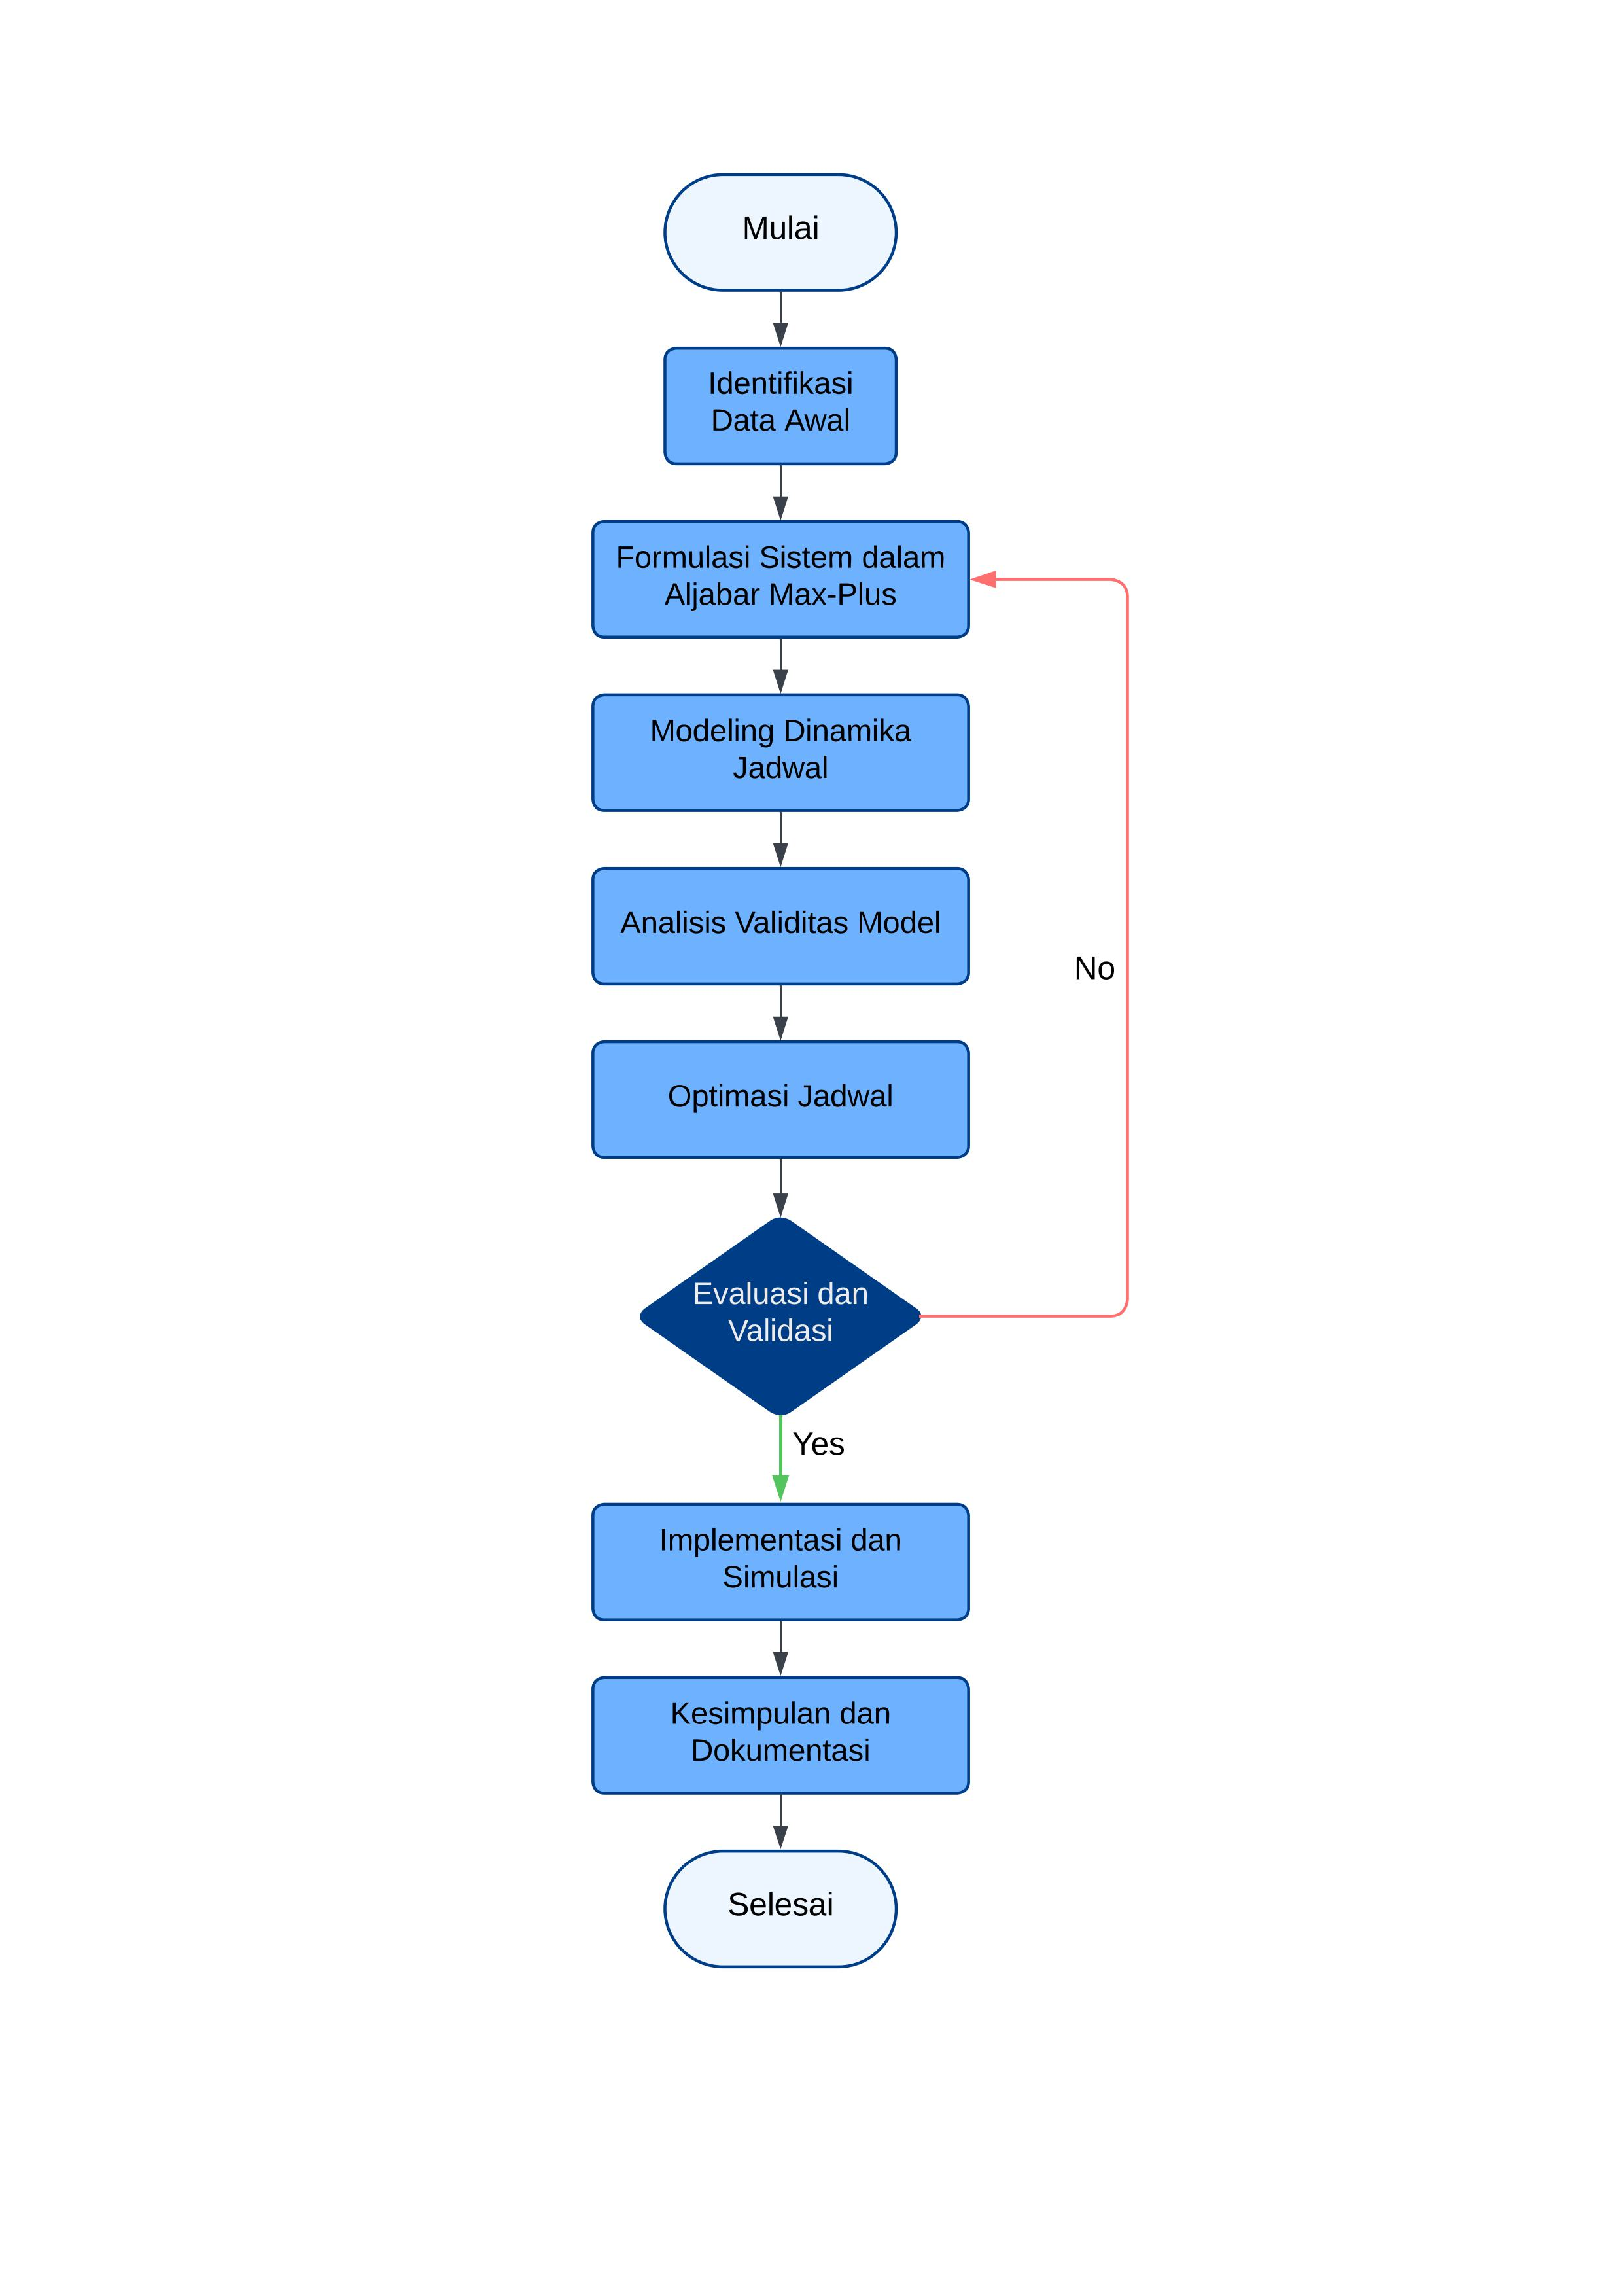
\includegraphics[trim={0 2cm 0 2cm},clip,scale=0.7]{foto/Diagram alir max plus.jpg}
	\caption{Diagram Alir Metodologi.}
	\label{diagramalir}
\end{figure}

\section{Identifikasi Data Awal}
Langkah pertama dalam penelitian ini adalah mengidentifikasi data awal yang relevan untuk membangun model. Data yang dikumpulkan meliputi parameter sistem yang akan digunakan dalam formulasi model serta pola waktu yang sesuai.

\section{Formulasi Sistem dalam Aljabar Max-Plus}
Setelah data awal diidentifikasi, sistem diformulasikan dalam kerangka aljabar Max-Plus. Langkah ini mencakup representasi elemen waktu dan operasi dalam bentuk matriks Max-Plus, yang mempermudah analisis dan optimasi jadwal.

\section{Modeling Dinamika Jadwal}
Berdasarkan formulasi Max-Plus, dinamika jadwal dimodelkan. Hal ini mencakup analisis perilaku sistem dalam berbagai kondisi input dan output, serta potensi pengaruh parameter waktu pada kinerja sistem.

\section{Analisis Validitas Model}
Langkah ini bertujuan untuk mengevaluasi validitas model yang telah dibangun. Apabila model tidak valid atau tidak sesuai dengan data dan sistem nyata, maka dilakukan perbaikan dan iterasi kembali ke tahap formulasi.

\section{Optimasi Jadwal}
Tahap berikutnya adalah melakukan optimasi terhadap jadwal berdasarkan model yang telah tervalidasi. Optimasi ini bertujuan untuk mencari solusi terbaik dalam penjadwalan yang sesuai dengan kriteria yang ditentukan.

\section{Evaluasi dan Validasi}
Hasil optimasi dievaluasi dan divalidasi untuk memastikan bahwa solusi yang diperoleh sesuai dengan tujuan penelitian. Jika evaluasi menunjukkan ketidaksesuaian, maka dilakukan revisi pada langkah sebelumnya.

\section{Implementasi dan Simulasi}
Setelah validasi berhasil, model diterapkan dan diuji melalui simulasi. Hasil simulasi akan memberikan gambaran tentang performa jadwal yang dioptimalkan dalam kondisi nyata.

\section{Kesimpulan dan Dokumentasi}
Langkah terakhir adalah merangkum hasil penelitian dalam bentuk kesimpulan dan mendokumentasikan seluruh proses dalam laporan tugas akhir.

\section{Jadwal Kegiatan}
Berikut ini disajikan tabel jadwal kegiatan yang akan dilakukan selama 3 bulan dan berkoresponden dengan metodologi.\vspace{0.5cm}

% Membuat tabel
\begin{table}[H]
\caption{Jadwal Kegiatan}
\centering
\begin{tabular}{|C{0.6cm}|L{5.7cm}|C{0.25cm}|C{0.25cm}|C{0.25cm}|C{0.25cm}|C{0.25cm}|C{0.25cm}|C{0.25cm}|C{0.25cm}|C{0.25cm}|C{0.25cm}|C{0.25cm}|C{0.25cm}|}
\hline
&&\multicolumn{12}{c|}{\textbf{BULAN}}\\\cline{3-14}
\multicolumn{1}{|c|}{\textbf{NO}}&\multicolumn{1}{c|}{\textbf{NAMA KEGIATAN}}&\multicolumn{4}{c|}{1}&\multicolumn{4}{c|}{2}&\multicolumn{4}{c|}{3}\\\cline{3-14}
&&1&2&3&4&1&2&3&4&1&2&3&4\\\cline{1-14}

1&Identifikasi Data Awal&\cellcolor{black!}&\cellcolor{black!}&&&&&&&&&&\\\hline
2&Formulasi Sistem dalam Aljabar Max-Plus&&&\cellcolor{black!}&\cellcolor{black!}&\cellcolor{black!}&&&&&&&\\\hline
3&Modeling Dinamika Jadwal&&&&&\cellcolor{black!}&\cellcolor{black!}&\cellcolor{black!}&&&&&\\\hline
4&Analisis Validitas Model&&&&&&&&\cellcolor{black!}&\cellcolor{black!}&\cellcolor{black!}&&\\\hline
5&Optimasi Jadwal&&&&&&&&\cellcolor{black!}&\cellcolor{black!}&\cellcolor{black!}&&\\\hline
6&Implementasi dan Simulasi&&&&&&&&&\cellcolor{black!}&\cellcolor{black!}&\cellcolor{black!}&\\\hline
7&Kesimpulan dan Dokumentasi&&&&&&&&&\cellcolor{black!}&\cellcolor{black!}&\cellcolor{black!}&\cellcolor{black!}\\\hline

\end{tabular}
\label{TabelJadwalKegiatan}
\end{table}
%%%%%%%%%%%%%%%%%%%%%%%%  Bab III  %%%%%%%%%%%%%%%5%%%%%%%%%%


%%%%%%%%%%%%%%%%%%%%%%%%  Dapus  %%%%%%%%%%%%%%%5%%%%%%%%%%

\pagebreak
\DaftarPustaka
%%%%%%%%%%%%%%%%%%%%%%%%  Dapus  %%%%%%%%%%%%%%%5%%%%%%%%%%
	
\end{document}